%\documentclass[12pt,a4paper,twoside]{article}
\documentclass[12pt,a4paper,oneside]{article}
\usepackage[latin1]{inputenc}
\usepackage{amssymb, amsmath, amsfonts, mathbbol}
\usepackage{graphics,graphicx,epsfig,ulem} 
\usepackage{multirow} % Allows multirow tables
\usepackage[margin=2.5cm]{geometry} % Set page margins
\usepackage{cite} % For better citations
\usepackage{url} % For better URLs
\usepackage{afterpage} % For flushing floats

% Fonts
\usepackage[T1]{fontenc}
\usepackage{cmbright}

% Double spacing
\usepackage{setspace}

% Headings
%\pagestyle{myheadings}
%\markboth{}{Running Coupling in the Standard Model and Beyond}

\begin{document}

\title{Running Coupling in the Standard Model and Beyond} 
\date{April 2011}
\author{Jonathan Arnold\thanks{Physics Department, University of Durham, South Road, Durham, DH1 3LE; e-mail correspondence to jonathan.arnold@durham.ac.uk} \\ Final Report for MPhys Physics (F301) \\ Supervisor: Dr. C. Maxwell}

\maketitle

%Start double spacing
\doublespace

\begin{abstract}
The running of the coupling strength with energy is analysed for the SU(3), SU(2) and U(1) sectors of the Standard Model, Minimal Supersymmetric Standard Model (MSSM) and Extra Dimension extensions to the MSSM to determine whether the sectors unify at high energy, admitting the possibility of a Grand Unified Theory (GUT). We find that the Standard Model does not admit unification. The Minimal Supersymmetric Standard Model admits a unification point at an energy $M_\mathrm{GUT} = 10^{(16.07 \pm 0.01)}$ GeV when the supersymmetry breaking scale $M_\mathrm{SUSY} = 10^{(3.37 \pm 0.01)}$ GeV, in agreement with previous papers. Adding compactified extra dimensions to the MSSM reduces the unification energy by 3 orders of magnitude to $\sim 10^{13}$ GeV, irrespective of the number of dimensions added; this value of $M_\mathrm{GUT}$ is not consistent with proton decay, and hence another mechanism (such as Kaluza-Klein selection rules) must be proposed to allow this.
\end{abstract}

\newpage
\tableofcontents

\newpage
\section{Introduction}

One of the greatest triumphs of 20th Century physics has been the Standard Model (SM). In it, the principle of local gauge invariance has been used to show that electromagnetic, strong and weak interactions can be modelled using the SU(3)$\times$SU(2)$\times$U(1) gauge groups to spectacular accuracy\cite{sm-1,sm-2}. Despite these great successes, it has become evident that the Standard Model does not describe a number of phenomena accurately, such as the observations of neutrino oscillations \cite{neutrinos}, matter-antimatter asymmetry \cite{mass} and the hierarchy problem \cite{hier}. As well as this, the somewhat large parameter space of the SM and large differences in the magnitude of these parameters has led some to argue that the theory is unnatural \cite{unnatural}. Due to these problems, it is reasonable to find an encompassing theory that includes the Standard Model within it and treat the Standard Model as a low-energy effective field theory, generalising to a more fundamental theory at higher energy.

To further fuel the hypothesis of a more fundamental theory, it has been widely noted \cite{amaldi, running-2} that the coupling strengths for the electromagnetic, strong and weak interactions vary (``run'') depending on the energy scale, due to renormalisation. The running of these couplings allows us to suggest that they would take the same value (``unify'') at a certain energy scale. If this unification exists then it admits the possibility of a Grand Unified Theory (GUT), capable of describing all three interactions of the SM as a single unified interaction at high energy. Thus, we can postulate that at this unification scale the physics associated with the `more fundamental theory' alluded to earlier becomes manifest.

One of the more popular theories for physics beyond the SM is the concept of supersymmetry; in this theory, the inclusion of a boson-fermion symmetry allows us to correct the hierarchy problem\footnote{More specifically, the MSSM refines the heirarchy problem into a ``little hierarchy problem'' \cite{lhp}.}. The most simple way of including supersymmetry in the SM is the Minimal Supersymmetric Standard Model (MSSM) \cite{mssm}. Supersymmetry is a `hot topic' recently as its predictions of superpartner particles should be observed in the next few years at the Large Hadron Collider \cite{mssm-lhc}.

As well as this, a number of groups have focussed on the role extra dimensions could potentially play on Nature \cite{ed-1, ed-2}. The introduction of extra dimensions is a natural extension of more fundamental theories, such as string theory \cite{string}. This paper pays particular attention to the use of compactified extra dimensions - extra dimensions that are only manifest at small distance scales - as it proposes unification at intermediate mass scales \cite{gherghetta}.

These theories are just some of a large number of GUTs that have been proposed \cite{pdg}; all require a unification point to exist, although how this unification is broken is theory-dependent.

This paper investigates the scales and conditions required to unify electromagnetism, strong and weak interactions into a single GUT, paying particular attention to the SM, MSSM and extensions to the MSSM that utilise compactified extra dimensions. In Section \ref{sec:rc} we outline how the process of renormalisation gives rise to running coupling. It also details the computational methods used in determining how the couplings run, as well as how various parameters in the theories are fixed during the investigation. Sections \ref{sec:sm}-\ref{sec:ed} then go into detail about how the couplings run in each theory as well as discussing the implications of each. Finally, in Section \ref{sec:conc} we draw conclusions from the entire investigation and outline further work in the field.

In this paper natural units $\hbar = c = 1$ are used throughout. The definition $\alpha = g^2 / 4 \pi$ (which is analogous to the fine structure constant in Quantum Electrodynamics) is also used.

\section{Running Coupling}
\label{sec:rc}

\subsection{Analytical Considerations}

\begin{figure}[!ht]
\begin{center}
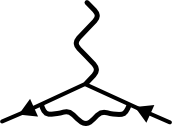
\includegraphics[width=3cm]{figs/vertex-1loop.png}
\caption[]{One-loop electron vertex: an example of a Feynman diagram that has a divergent amplitude. Using regularisation and renormalisation this amplitude becomes finite.}
\label{fig:vertex}
\end{center}
\end{figure}

Almost all theories of interaction in particle physics admit solutions where infinities become problematic at high energy (also known as the ultraviolet region). This occurs usually when one or more `loops' are added to a Feynman diagram; for example, the one-loop contribution to the electron vertex in Quantum Electrodynamics (QED) diverges as the loop photon energy increases (see Figure \ref{fig:vertex}). 

In order to combat these anomalies, we use two mathematical tools. The first, \textit{regularisation}, introduces the concept of a regulator. At high energies, this regulator ensures that the integral remains finite, and in the low energy limit the regulator vanishes. There is more than one scheme for regularisation and the choice of scheme is somewhat arbitrary, depending on the theory \cite{peskin}. In this paper will use two schemes - the modified Minimal Subtraction scheme ($\overline{\mathrm{MS}}$) \cite{ms} for the SM and Dimensional Regularisation ($\overline{\mathrm{DR}}$) \cite{dr} for the MSSM.

Regularisation can still lead to divergent integrals; we therefore use it together with the process of \textit{renormalisation}. This process uses a scale symmetry argument to suggest that the `bare' parameters used in equations are different to values we determine from experiment, and that they are related by an expression that depends on the energy scale involved. In the case of electromagnetism, this has a physical argument: the bare charge around, for example, an electron is screened by a cloud of net negative charge formed from vacuum particle-antiparticle pairs being attracted to the electron; this increases its \textit{effective } interaction strength \cite{renorm-2}.

Using a procedure outlined by \textit{Bogoliubov and Shirkov} \cite{bogoliubov}, we can use regularisation and renormalisation to ensure that all divergent integrals in our theory are finite (assuming our theory is renormalisable). As a result of this procedure, we find that the coupling `constant' associated with the strength of a particular interaction is no longer constant, but varies (``runs'') with energy. We can characterise this variation with the \textit{beta function}: the strength of an interaction $g$ at a certain scale $\mu$ is given by
\begin{equation}
\beta (\mu) = \mu \frac{\partial g}{\partial \mu} \:.
\label{eqn:beta}
\end{equation}

The beta function is dependent on the theory we consider, and provides us with a differential equation that we can solve (computationally, or in some cases analytically) to give the value of the coupling strength at a certain energy scale. It is more useful to have an equation of the form
\[
\mu \frac{d}{d \mu} \alpha^{-1} (\mu) = \ldots \:,
\]
(where $\alpha = g^2 / 4 \pi$) which can be easily derived from Eq. \ref{eqn:beta}. Equations of this form are typically referred to as renormalisation group (RG) equations.

In the theories considered by this paper we will have three differential equations to solve, for the SU(3), SU(2) and U(1) sectors respectively; we thus adopt an index notation

\begin{equation}
\mu \frac{d}{d \mu} \alpha^{-1}_i (\mu) = \ldots \:,
\label{eqn:rg-i}
\end{equation}
where $i = 1, 2, 3$ denotes the U(1), SU(2) and SU(3) sectors respectively. By solving Eq. \ref{eqn:rg-i} at several energies we can determine how the couplings run with energy, as well as whether the couplings unify at any point.

\subsection{Computational Investigation}
\label{sec:comp}

In this paper we solve RG equations of the form given in Eq. \ref{eqn:rg-i} computationally using two different integration methods: for more information, see Appendix \ref{apx:tic}. 

As with any series of first-order differential equations, we must define initial conditions: one for each differential equation. In this project, we focussed on two particular types of initial conditions: the first, herein referred to as the \textit{forward propagation} (FP) method, fixes the initial values of $\alpha_i^{-1}(M_Z)$ using data from the \textit{Particle Data Group} \cite{pdg} and propagates forward from these values to determine the unification point, if one exists. 

We can define the \textit{unification point} ($M_\mathrm{GUT}$, $\alpha_\mathrm{GUT}$) as the energy scale $\mu$ and average coupling strength $\overline{\alpha}(\mu)$ that minimise
\begin{equation}
\overrightarrow{\chi}^2 (\mu) = \frac{1}{3} \sum_{i = 1}^{3} \left(\dfrac{\alpha_i^{-1}(\mu) - \overline{\alpha^{-1}}(\mu)}{\sigma[\alpha_i^{-1}(M_Z)]}\right)^2 \:,
\label{eqn:fp}
\end{equation}
where $\sigma[\alpha_i^{-1}(M_Z)]$ is the error in $\alpha_i^{-1}$ at $M_Z$, calculated in Appendix \ref{apx:errors}. In this method, we define the value of $\overrightarrow{\chi}^2$ at the unification point as $\overrightarrow{\chi}^2_\mathrm{min}$. $\overrightarrow{\chi}^2$ gives a useful indicator of how well unified a model is: if $\overrightarrow{\chi}_\mathrm{min}^2 \leq 1$ then unification has occurred within error.

The alternative set of initial conditions, herein referred to as \textit{backward propagation} (BP), fixes a unification point (with unification strength $\alpha_\mathrm{GUT}$ and unification energy $M_\mathrm{GUT}$) and propagates backwards from this value to $M_Z$ to determine how close the couplings are to experimental values. 

This change in initial conditions also changes how we quantise unification:
\begin{equation}
\overleftarrow{\chi}^2 = \frac{1}{3} \sum_{i = 1}^{3} \left(\dfrac{\alpha_{i,\mathrm{calc}}^{-1}(M_Z) - \alpha_{i,\mathrm{exp}}^{-1}(M_Z)}{\sigma[\alpha_{i,\mathrm{exp}}^{-1}(M_Z)]}\right)^2 \:.
\label{eqn:bp}
\end{equation}
Here, all values of $\alpha_i$ are evaluated at $M_Z$. As with traditional $\chi^2$ analysis, we take the difference of the theoretical predictions and experimental values, then divide by the error in the experimental value. Although the initial conditions have changed, the unification condition $\overleftarrow{\chi}^2 \leq 1$ remains. 

The majority of theories discussed in this paper result in running couplings that depend on one or more \textit{free parameters}: for example, in any BP analysis $M_\mathrm{GUT}$ and $\alpha_\mathrm{GUT}$ are free to vary. When a theory admits one free parameter we simply step across all admissible values of the free parameter to find the minimum value of $\chi^2$ (i.e. gives best unification). When there is more than one free parameter we use a hybrid method of convergence - which we entitled the Monte-Carlo Levenberg-Marquardt algorithm, or MCLM algorithm - to determine quickly the values of the free parameters that give the minimum value of $\chi^2$. (A full discussion of the MCLM algorithm is contained in Appendix \ref{apx:mclm})

The FP method gives us a rough idea of whether the couplings will unify at high energy. We can see that the FP method will always have two less free parameters than a BP method of the same model ($M_\mathrm{GUT}$ and $\alpha_\mathrm{GUT}$ are added to the BP method); for this reason, we expect $\overleftarrow{\chi}^2 < \overrightarrow{\chi}^2_\mathrm{min}$; however, it should be noted that the BP method does require unification to be at least approximately found from a FP analysis - obviously it is not reasonable to assume total unification if the theory does not approximately unify!

All examples and graphs were written and produced in the Python programming language, making heavy use of the module \texttt{numpy} \cite{scipy} for array handling and manipulation, \texttt{scipy} \cite{scipy} for solving differential equations and \texttt{pylab} (also known as \texttt{matplotlib}) \cite{pylab} for plotting.

\section{Standard Model (SM)}
\label{sec:sm}

\subsection{Theory}

The Standard Model models three fundamental interactions using an SU(3)$\times$SU(2)$\times$U(1) gauge groups and the principle of local gauge invariance to form a quantum field theory \cite{sm}. For each of these interactions we associate a coupling strength to it. We also suggest that there is no new physics in the `desert' between our current experimental bounds (around $10^3$ GeV) and higher energy.

The SM is renormalisable \cite{sm-renorm}, and so we are able to determine a beta-function for it. We repeat the procedure outlined by \textit{Amaldi et al.} \cite{amaldi}: we define the couplings as
\begin{equation}
\alpha_1^{-1} = \dfrac{3}{5} \dfrac{\cos^2 \theta_W}{\alpha_\mathrm{EM}} \:, \quad
\alpha_2^{-1} = \dfrac{\sin^2 \theta_W}{\alpha_\mathrm{EM}} \:, \quad
\alpha_3^{-1} = \dfrac{1}{\alpha_s}
\label{eqn:coupling-def}
\end{equation}
where $\alpha_\mathrm{EM}$, $sin^2 \theta_W$ and $\alpha_s$ are the fine-structure constant, weak mixing angle and strong coupling constant respectively (all experimentally determined parameters), and we include the $3/5$ factor in the definition of $\alpha_1^{-1}$ to ensure normalization at the unification point\footnote{Specifically, we require that the generators of the SU(2) and U(1) sectors have equal traces due to them both lying in a single representation of a (simple) group: $\mathrm{Tr}(\frac{1}{4} Y^2) = \mathrm{Tr}((T^3)^2)$, where $Y$ and $T^3$ are the U(1) and SU(2) generators respectively; as $\mathrm{Tr}(\frac{1}{4} Y^2) / \mathrm{Tr}((T^3)^2) = \frac{5}{3}$, we renormalise $\alpha_\mathrm{EM}$ by this factor and the requirement is satisfied \cite{5thirds}.}. 

Using the world-averaged values from the \textit{Particle Data Group} \cite{pdg} 
\begin{align}
\alpha_\mathrm{EM}^{-1} (M_Z) &= 127.91 \pm 0.02 \nonumber \\
\sin^2 \theta_W (M_Z) &= 0.2312 \pm 0.0002 \label{eqn:world-vals} \\
\alpha_s (M_Z) &= 0.119 \pm 0.002 \nonumber
\end{align}
we find
\begin{equation}
\alpha_1^{-1} (M_Z) = 59.00 \pm 0.03 \:, \quad
\alpha_2^{-1} (M_Z) =  29.52 \pm 0.03 \:, \quad
\alpha_3^{-1} (M_Z) =  8.3 \pm 0.1
\label{eqn:couplingvals}
\end{equation}
where the errors on these parameters are propagated using the procedure in Appendix \ref{apx:errors}. 
We consider one- and two-loop contributions to the beta function, corresponding to the contributions of Feynman diagrams with one loop and two loops within them respectively. Using these definitions, we find that \cite{amaldi}
\[
\mu \dfrac{d}{d \mu} \alpha_i (\mu) = \dfrac{1}{2 \pi} \left( b^\mathrm{SM}_i + \sum_{j=1}^{3} \dfrac{b^\mathrm{SM}_{i j}}{4 \pi} \alpha_j (\mu) \right) \alpha_i^2 (\mu) \:.
\]
This is rearranged to give
\begin{equation}
\mu \dfrac{d}{d (\ln \mu)} \alpha_i^{-1} (\mu) = -\dfrac{1}{2 \pi} \left( b^\mathrm{SM}_i + \sum_{j=1}^{3} \dfrac{b^\mathrm{SM}_{i j}}{4 \pi} \alpha_j (\mu) + \mathcal{O}(\alpha_j^2) \right) \:,
\label{eqn:sm-beta}
\end{equation}
where we adopt ``big O'' notation to denote higher order terms. Although the form is similar for all three sectors of the model, the constants ($b^\mathrm{SM}_i$ and $b^\mathrm{SM}_{ij}$ at one- and two-loop level respectively) are not: for the SM\cite{b},
\singlespace % Conserve the space!
\begin{align}
b^\mathrm{SM}_i &= 
\begin{pmatrix} 0 \\ -\frac{22}{3} \\ -11 \end{pmatrix} 
+ N_\mathrm{Fam} \begin{pmatrix} \frac{4}{3} \\ \frac{4}{3} \\ \frac{4}{3} \end{pmatrix} 
+ N_\mathrm{Higgs} \begin{pmatrix} \frac{1}{10} \\ \frac{1}{6} \\ 0 \end{pmatrix} \nonumber \\
b^\mathrm{SM}_{ij} &= 
\begin{pmatrix} 
0 & 0 & 0 \\ 
0 & -\frac{136}{3} & 0 \\ 
0 & 0 & -102 
\end{pmatrix}
+ N_\mathrm{Fam} 
\begin{pmatrix} 
\frac{19}{15} & \frac{3}{5} & \frac{44}{15} \\ 
\frac{1}{5} & \frac{49}{3} & 4 \\ 
\frac{11}{30} & \frac{3}{2} & \frac{76}{3}
\end{pmatrix}
+ N_\mathrm{Higgs}
\begin{pmatrix}
\frac{9}{50} & \frac{9}{10} & 0 \\
\frac{3}{10} & \frac{13}{6} & 0 \\
0 & 0 & 0
\end{pmatrix} 
\nonumber
\end{align}
\\
\doublespace
For the SM, we set the number of families of matter $N_\mathrm{Fam} = 3$ and the number of Higgs doublets $N_\mathrm{Higgs} = 1$:
\singlespace
\begin{equation}
b^\mathrm{SM}_i = 
\begin{pmatrix} \frac{41}{10} \\ -\frac{175}{6} \\ -7 \end{pmatrix}
\quad,\quad
b^\mathrm{SM}_{ij} = 
\begin{pmatrix} 
\frac{199}{50} & \frac{27}{10} & \frac{44}{5} \\ 
\frac{9}{10} & \frac{35}{6} & 12 \\ 
\frac{11}{10} & \frac{9}{2} & -26
\end{pmatrix}
\label{eqn:sm-bi-bij}
\end{equation}
\\
\doublespace
It is noted that there are no free parameters in this theory: because of this, we cannot `fine-tune' the theory to give unification - it will either give unification or it will not.

\subsection{Results and Discussion}

\begin{figure}[th]
\begin{center}
\begin{tabular}{cc}
(a) 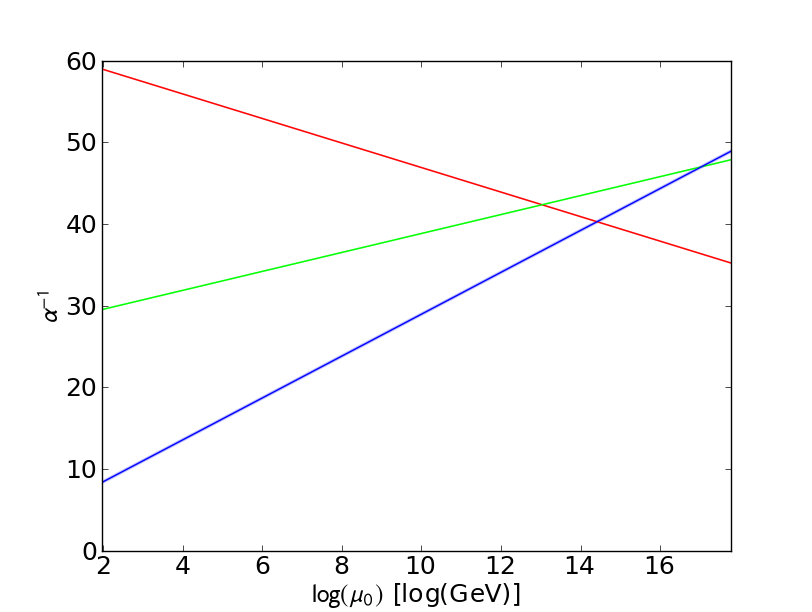
\includegraphics[width=6.85cm]{figs/sm-1loop.png} & (b) 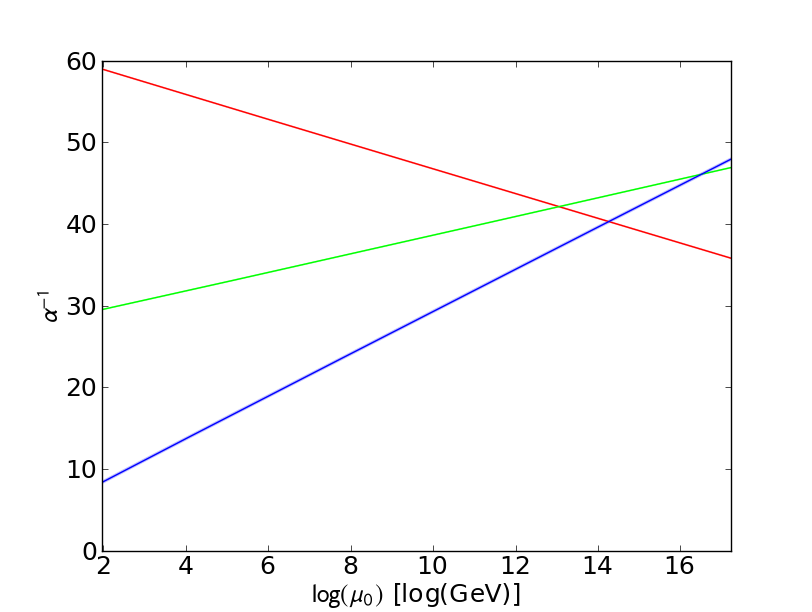
\includegraphics[width=6.85cm]{figs/sm-2loop.png} \\
\\
\multicolumn{2}{c}{
\begin{tabular}{l|cc|r}
Model & $M_\mathrm{GUT}$ [log(GeV)] & $\alpha^{-1}_\mathrm{GUT}$ & $\overrightarrow{\chi}^2 (M_\mathrm{GUT})$ \\
\hline
1-loop (a) & 13.63 & 40.94 & 2447 \\
2-loop (b) & 13.60 & 40.89 & 1878 \\
\end{tabular}
}

\end{tabular}

\caption[]{Graphs of $\alpha_1$ (red line, top at $\mu = M_Z$), $\alpha_2$ (green) and $\alpha_3$ (blue, bottom at $\mu = M_Z$) in the SM obtained by solving Eq. \ref{eqn:sm-beta} with the forward propagation (FP) method, together with a table detailing the results of quantising the amount of unification, as defined in the text. All values in the table are to 4 significant figures. (a) Considering 1-loop contributions to the SM beta function (b) Considering 1- and 2-loop contributions. As can be seen from the graphs and values of $\overrightarrow{\chi}^2 (M_\mathrm{GUT})$, no unification point exists for the SM up to 2 loops.}
\label{fig:sm}
\end{center}
\end{figure}

The FP method was used to solve Eq. \ref{eqn:sm-beta}; Figure \ref{fig:sm}a shows the results of considering only one-loop contributions (terms involving $b_i^\mathrm{SM}$ only), and Figure \ref{fig:sm}b shows the results of considering one- and two-loop contributions. Also included in Figure \ref{fig:sm} is a table showing the analysis of unification (as defined in Eq. \ref{eqn:fp}).

We can conclude from Figure \ref{fig:sm} that the SM does not admit unification by a large margin ($\overrightarrow{\chi}^2 \gg 1$). Inclusion of higher-order terms to the beta function would not improve unification, as the effect of each higher order decreases; one- and two-loop contributions are essentially the only contributions worth considering \cite{amaldi}. This also implies that using the BP method for the SM will not give reasonable results, as the method requires at least approximate unification to begin with. Obviously, if we consider unification to be true we require physics beyond the SM to explain it.

\section{Minimal Supersymmetric Standard Model (MSSM)}
\label{sec:mssm}

\subsection{Theory}

Supersymmetry is the postulation that there exists a transformation $Q$ that turns a bosonic state into a fermionic state:
\[
Q \vert{\mathrm{Boson}}\rangle = \vert{\mathrm{Fermion}}\rangle \:, \quad\quad Q \vert{\mathrm{Fermion}}\rangle = \vert{\mathrm{Boson}}\rangle
\]
As a corollary of this transformation, each particle in the Standard Model (quark, lepton or gauge boson) gains a \textit{superpartner} that it transforms into via $Q$ (squark, slepton, gaugino), existing in a \textit{supermultiplet} of Q \cite{mssm}. If no additional supermultiplets are included, we arrive at the Minimal Supersymmetric Standard Model (MSSM).

No conclusive evidence of supersymmetry has been found at low energy\footnote{Evidence of supersymmetry is predicted at the Large Hadron Collider, at energies just above our current experimental bounds \cite{mssm-lhc}.}; we therefore need to provide a way of breaking supersymmetry at low energy to incorporate this. We introduce this with a \textit{supersymmetry breaking scale} $M_\mathrm{SUSY}$, which must be above our experimental bounds. Below $M_\mathrm{SUSY}$ we assume no supersymmetry and that the running of the coupling is governed by the SM beta function, and above it we use the beta function for the MSSM\footnote{We expect a more subtle transition into supersymmetry; this is a simpler way of introducing supersymmetry and we believe that this retains the relevant physics \cite{amaldi}.}. 

Despite the inclusion of a number of new particles the differences between the SM and the MSSM are subtle when determining the running of the couplings. The couplings are offset very slightly, due to the difference in renormalisation scheme \cite{amaldi}:
\[
\frac{1}{\alpha_i^{\overline{\mathrm{DR}}}} = \frac{1}{\alpha_i^{\overline{\mathrm{MS}}}} - \frac{C_i}{12 \pi} \:,
\]
where $C_i$ are the quadratic Casimir coefficients of each group ($C_i = N$ for SU($N$) and $C_i = 0$ for U(1)). 

The RG equations decribing the three interactions retain the same form in the MSSM \cite{b, mssm-renorm}:
\begin{equation}
\mu \dfrac{d}{d (\ln \mu)} \alpha_i^{-1} (\mu) = -\dfrac{1}{2 \pi} \left( b^\mathrm{MSSM}_i + \sum_{j=1}^{3} \dfrac{b^\mathrm{MSSM}_{i j}}{4 \pi} \alpha_j (\mu) + \mathcal{O}(\alpha_j^2) \right) \quad\quad (\mu \geq M_\mathrm{SUSY})
\label{eqn:mssm-beta}
\end{equation}
Only the coefficients $b^\mathrm{MSSM}_i$ and $b^\mathrm{MSSM}_{i j}$ change:
\singlespace
\begin{align}
b^\mathrm{MSSM}_i &= 
\begin{pmatrix} 0 \\ -6 \\ -9 \end{pmatrix} 
+ N_\mathrm{Fam} \begin{pmatrix} 2 \\ 2 \\ 2 \end{pmatrix} 
+ N_\mathrm{Higgs} \begin{pmatrix} \frac{3}{10} \\ \frac{1}{2} \\ 0 \end{pmatrix} \nonumber\\
b^\mathrm{MSSM}_{ij} &= 
\begin{pmatrix} 
0 & 0 & 0 \\ 
0 & -24 & 0 \\ 
0 & 0 & -54
\end{pmatrix}
+ N_\mathrm{Fam} 
\begin{pmatrix} 
\frac{38}{15} & \frac{6}{5} & \frac{88}{15} \\ 
\frac{2}{5} & 14 & 8 \\ 
\frac{11}{15} & 3 & \frac{68}{3}
\end{pmatrix}
+ N_\mathrm{Higgs}
\begin{pmatrix}
\frac{9}{50} & \frac{9}{10} & 0 \\
\frac{3}{10} & \frac{7}{2} & 0 \\
0 & 0 & 0
\nonumber
\end{pmatrix} 
\end{align}
\\
\doublespace
In order to maintain the boson-fermion symmetry in the MSSM, we require a new Higgs doublet \cite{mssm}; hence, we use $N_\mathrm{Higgs}$ = 2, as well as $N_\mathrm{Fam} = 3$ as in the SM:
\singlespace
\begin{equation}
b^\mathrm{MSSM}_i = 
\begin{pmatrix} \frac{33}{5} \\ 1 \\ -3 \end{pmatrix}
\quad,\quad
b^\mathrm{MSSM}_{ij} = 
\begin{pmatrix} 
\frac{199}{25} & \frac{27}{5} & \frac{88}{5} \\ 
\frac{9}{5} & 25 & 24 \\ 
\frac{11}{5} & 9 & 14
\end{pmatrix}
\label{eqn:mssm-bi-bij}
\end{equation}
\\
\doublespace
We must also define new initial conditions for this system of differential equations: we introduce the constraint that $\alpha^{-1}_i (M_\mathrm{SUSY})$ must be the same for both the SM (Eq. \ref{eqn:sm-beta}) and MSSM (Eq. \ref{eqn:mssm-beta}) beta functions.

Higgs Yukawa couplings are known to contribute to the beta function at two-loop level: however, it has been noted that the effect of these couplings has little effect on the running of the couplings, and adds extra parameters to the theory \cite{yukawa}; as such, our treatment ignores Yukawa coupling.

$M_\mathrm{SUSY}$ is the single free parameter for this theory (using the FP method). By its definition we can set limits on its value: as we have not experimentally found evidence for supersymmetry at current particle accelerators, we know that $M_\mathrm{SUSY} > 10^3$ GeV. If we use the BP method we have three free parameters ($M_\mathrm{SUSY}$, $M_\mathrm{GUT}$ and $\alpha_\mathrm{GUT}^{-1}$) and therefore require a multidimensional convergence algorithm to find the optimal values.  We hence solve Eq. \ref{eqn:mssm-beta} using the MCLM algorithm, as discussed earlier in Section \ref{sec:comp} and in Appendix \ref{apx:mclm}.

We can constrain $M_\mathrm{GUT}$ and $\alpha_\mathrm{GUT}$ by requiring they do not violate the current experimental observations on proton decay; in the MSSM, the proton lifetime $\tau_p$ is related to $M_\mathrm{GUT}$ and $\alpha_\mathrm{GUT}$ by \cite{amaldi}
\begin{equation}
\tau_p \approx \frac{1}{\alpha_\mathrm{GUT}^2} \frac{M_\mathrm{GUT}^4}{M_p^5} \:.
\label{eqn:proton}
\end{equation}
Using data from the \textit{Particle Data Group} \cite{pdg},
\[
M_p = 0.93827201 \:\mathrm{GeV} \quad,\quad \tau_p > 2.1 \times 10^{29} \:\mathrm{years} \:,
\]
this implies that
\begin{equation}
\alpha_\mathrm{GUT}^{-1} M_\mathrm{GUT}^2 > \sqrt{\tau_p M_p^5} \quad\Rightarrow\quad \alpha_\mathrm{GUT}^{-1} M_\mathrm{GUT}^2 > 1.08 \times 10^{30} \:\mathrm{GeV}^2
\label{eqn:proton-limit}
\end{equation}

\subsection{Results and Discussion}

\begin{figure}[p]
\begin{center}
(a) 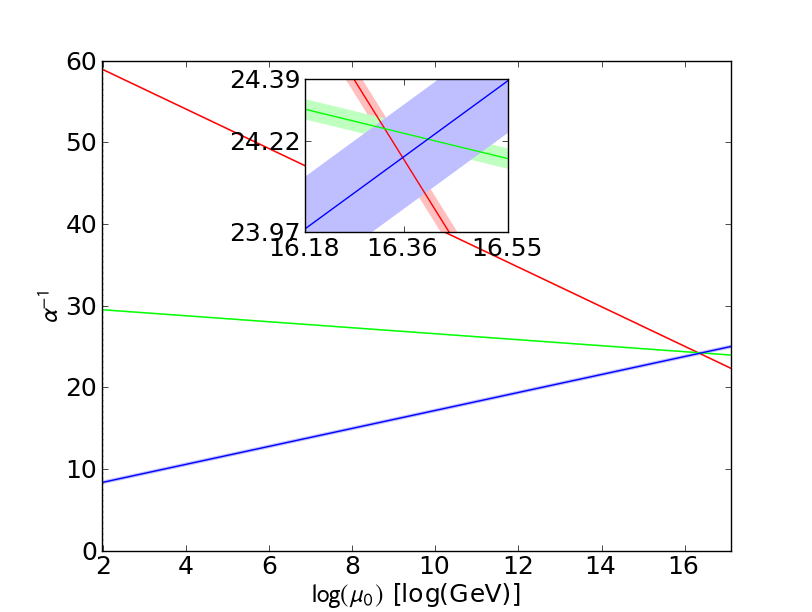
\includegraphics[width=9cm]{figs/mssm-1loop.png} \\
(b) 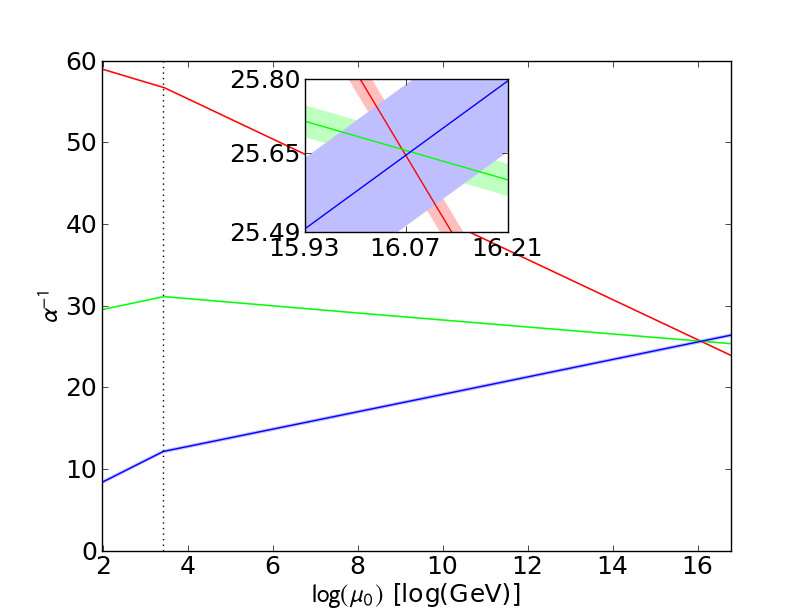
\includegraphics[width=9cm]{figs/mssm-2loop.png} \\
\vspace{2em}
\begin{tabular}{l|c|cc|r}
Model & $M_\mathrm{SUSY}$ [log(GeV)] & $M_\mathrm{GUT}$ [log(GeV)] & $\alpha^{-1}_\mathrm{GUT}$ & $\overrightarrow{\chi}^2 (M_\mathrm{GUT})$ \\
\hline
1-loop (a) & 0 & 16.3 & 24.2 & 0.960 \\
2-loop (b) & $3.4\pm0.1$ & 16.1 & 25.6 & 0.0206 \\
\end{tabular}

\caption[]{Plot of $\alpha_1$ (red line, top at $\mu = M_Z$), $\alpha_2$ (green) and $\alpha_3$ (blue, bottom at $\mu = M_Z$) in the MSSM obtained by solving Eq. \ref{eqn:mssm-beta} with the forward propagation (FP) method, together with a table detailing the results of quantising the amount of unification, as defined in the text. The value of $M_\mathrm{SUSY}$ (dashed vertical line, Figure \ref{fig:mssm-fp}b) was set to minimise the value of $\overrightarrow{\chi}^2 (M_\mathrm{GUT})$ . All values except $M_\mathrm{SUSY}$ in the table are to 3 significant figures when $M_\mathrm{SUSY}$ takes its central value. (a) Considering 1-loop contributions to the MSSM beta function (b) Considering 1- and 2-loop contributions. Experimental errors are shown as lightly shaded regions around the central value. It is noted that that the 1-loop value for $M_\mathrm{SUSY}$ is unphysical - see text for more details.}
\label{fig:mssm-fp}
\end{center}
\end{figure}

As done with the SM, Eq. \ref{eqn:mssm-beta} was solved using the FP method. The value of $M_\mathrm{SUSY}$ was set to the value at which $\overrightarrow{\chi}^2 (M_\mathrm{GUT})$ was minimised (i.e. gave the best unification). The results of this analysis are shown in Figure \ref{fig:mssm-fp}: Figure \ref{fig:mssm-fp}a shows a 1-loop analysis (only considering $b_i^\mathrm{MSSM}$ terms in Eq. \ref{eqn:mssm-beta}) and Figure \ref{fig:mssm-fp}b shows a 2-loop analysis (considering both $b_i^\mathrm{MSSM}$ and $b_{ij}^\mathrm{MSSM}$ terms). A table of values corresponding to the minimum of $\overrightarrow{\chi}^2 (M_\mathrm{GUT})$ is also found in Figure \ref{fig:sm}.

At both one- and two-loop contributions the MSSM unifies ($\overrightarrow{\chi}^2 < 1$) at an energy scale $\sim 10^{16}$ GeV, well within experimental bounds from proton decay. However, at 1-loop best unification is found when $M_\mathrm{SUSY} = 0$: this is obviously an unphysical result, as we do not see any experimental signatures of supersymmetry at our current experimental energy ranges. The two-loop analysis heals our problem by placing $M_\mathrm{SUSY}$ at an energy scale just outside of our current experimental limits: it is anticipated that the Large Hadron Collider at CERN will address the energy range around the value of $M_\mathrm{SUSY}$ predicted here \cite{lhc-1, lhc-2}.

\begin{figure}[t]
\begin{center}
\begin{tabular}{cc}
(a) 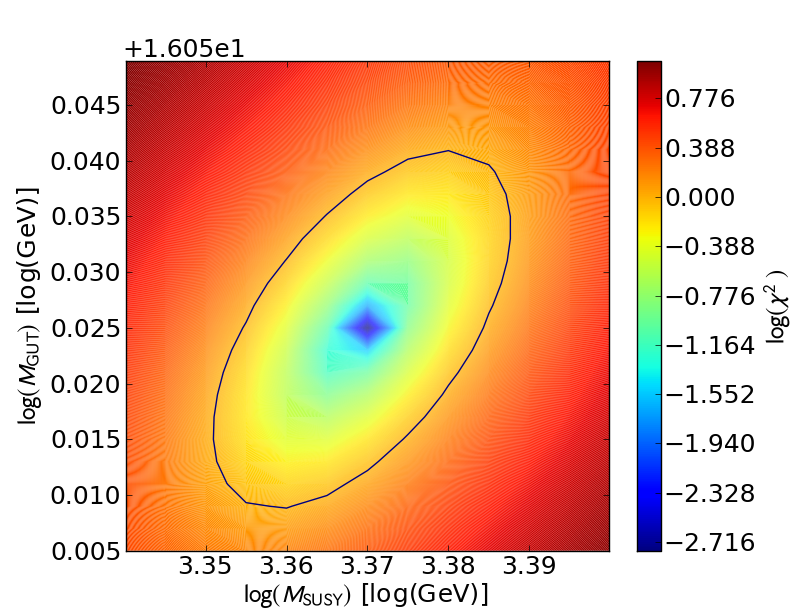
\includegraphics[width=6.85cm]{figs/mssm-contour-fix-ainv.png} &
(b) 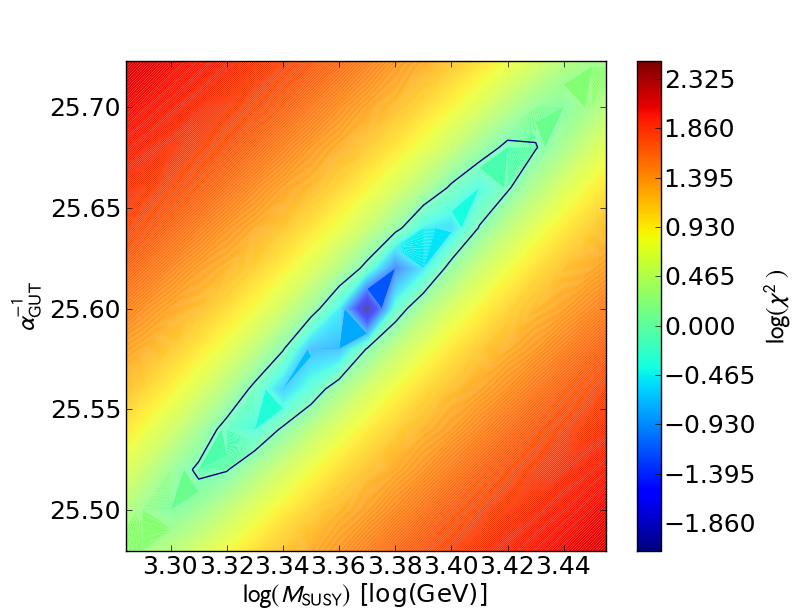
\includegraphics[width=6.85cm]{figs/mssm-contour-fix-mgut.png} \\
\multicolumn{2}{c}{(c) 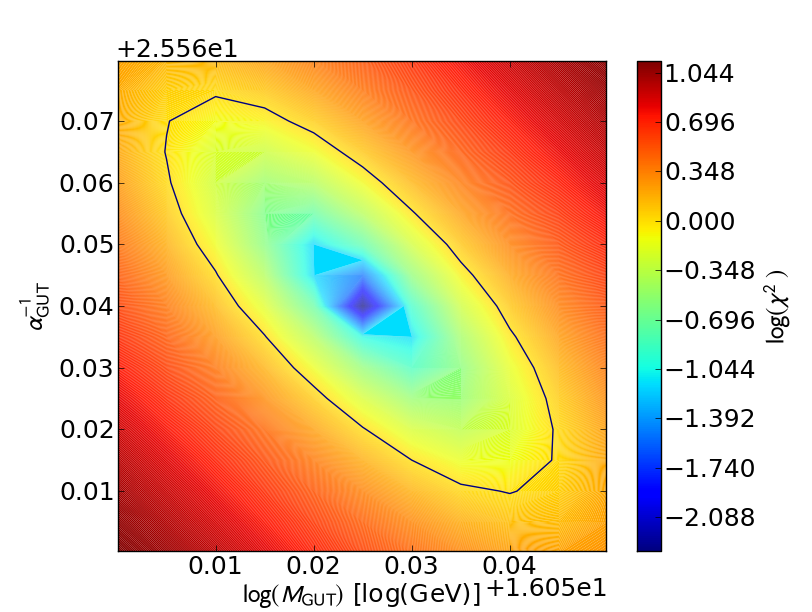
\includegraphics[width=6.85cm]{figs/mssm-contour-fix-msusy.png}} \\
\end{tabular}

\caption[]{Surfaces showing the variation in $\overleftarrow{\chi}^2$ with respect to the free parameters $\alpha_\mathrm{GUT}^{-1}$, $M_\mathrm{GUT}$ and $M_\mathrm{SUSY}$ involved in the BP method of solving the two-loop MSSM beta function. In each of the plots one of the parameters is fixed to the values given in Figure \ref{fig:mssm-bp} and the other two are are allowed to vary. (a) $\alpha_\mathrm{GUT}^{-1}$ fixed, (b) $M_\mathrm{GUT}$ fixed, (c) $M_\mathrm{SUSY}$ fixed. The contour (black line) encloses the area where $\overleftarrow{\chi}^2 < 1$. The minimum values of $\overleftarrow{\chi}^2$ in these plots are limited by the plots' resolution: in fact, $\overleftarrow{\chi}^2 \rightarrow 0$ (see the text and Figure \ref{fig:mssm-bp} for more details). }
\label{fig:mssm-bp-chi2}
\end{center}
\end{figure}

\begin{figure}[t]
\begin{center}
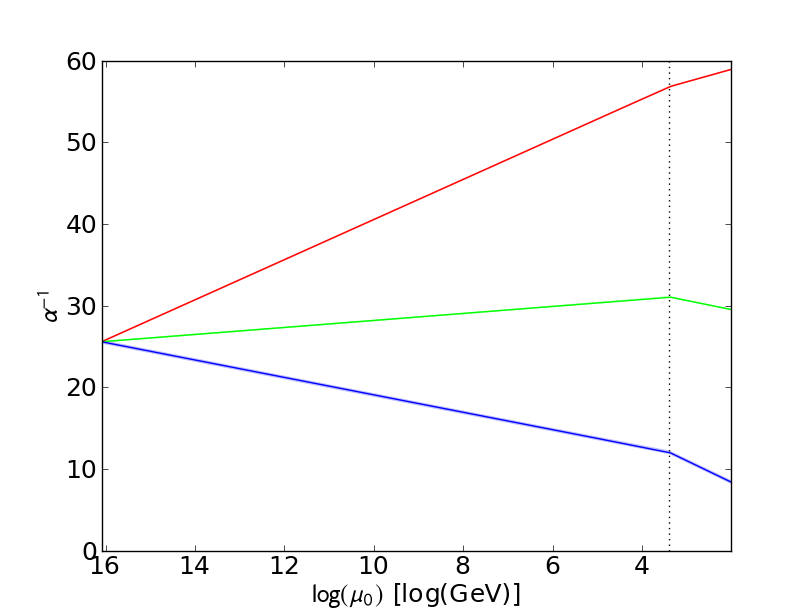
\includegraphics[width=9cm]{figs/mssm-bp-2loop.png} \\
\vspace{2em}
\begin{tabular}{ccc|c}
$M_\mathrm{SUSY}$ [GeV] & $M_\mathrm{GUT}$ [GeV] & $\alpha_\mathrm{GUT}^{-1}$ & $\overleftarrow{\chi}^2$ \\
\hline
$10^{(3.37\pm0.01)}$  & $10^{(16.07\pm0.01)}$ & $25.60\pm0.02$ & $< 0.01$
\end{tabular}

\caption[]{Plot of $\alpha_1$ (red line, top at $\mu = M_Z$), $\alpha_2$ (green) and $\alpha_3$ (blue, bottom at $\mu = M_Z$) in the MSSM using the backward propagation (BP) method, and a table of parameters used to produce the plot. $M_\mathrm{SUSY}$ (dashed vertical line), $M_\mathrm{GUT}$ and $\alpha_\mathrm{GUT}^{-1}$ are allowed to vary to minimise $\overleftarrow{\chi}^2$: the values giving a minimum $\overleftarrow{\chi}^2$ are shown in the table and plotted. Errors were calculated by minimising $| \overleftarrow{\chi}^2 + 1 |$, leaving all but the parameter in question fixed. The value of $\overleftarrow{\chi}^2$ in the table is the value determined when the central values of $M_\mathrm{SUSY}$, $M_\mathrm{GUT}$ and $\alpha_\mathrm{GUT}^{-1}$ are taken to 2 decimal places; by specifying more, $\overleftarrow{\chi}^2$ can be as low as $10^{-12}$: see text for details.}
\label{fig:mssm-bp}
\end{center}
\end{figure}

As unification occurs in both FP analyses (within tolerance: $\overrightarrow{\chi}^2 (M_\mathrm{GUT}) < 1$), it is reasonable to use the BP method. Figure \ref{fig:mssm-bp-chi2} shows how the value of $\overleftarrow{\chi}^2$ varies with respect to each of the free parameters $M_\mathrm{SUSY}$, $M_\mathrm{GUT}$ and $\alpha_\mathrm{GUT}^{-1}$, and Figure \ref{fig:mssm-bp} shows the results of minimising $\overleftarrow{\chi}^2$ using the MCLM algorithm.

As we have as many free parameters as equations (3), we can obtain perfect agreement with experimental results - we have only reported $\overleftarrow{\chi}^2 < 0.01$ due to error bars, but from further analysis this value can be lower: for example, when
\singlespace
\[
M_\mathrm{SUSY} = 10^{3.36825754} \:\mathrm{GeV} \:,\quad M_\mathrm{GUT} = 10^{16.07515093} \:\mathrm{GeV} \:, \quad \alpha_\mathrm{GUT}^{-1} = 25.59902942 \:,
\]
\[
\Rightarrow \overleftarrow{\chi}^2 \sim 10^{-12} \:.
\]
\doublespace
In theory, $\overleftarrow{\chi}^2$ can be as close to 0 as we require. Despite this `under-constraint', The values for the free parameters are in agreement with the FP analysis, within error: this further suggests that our analysis is not flawed, as now two different methods of determining parameter values have arrived at similar values. The BP analysis has also allowed us to further constrain the values of each of the parameters with an error, calculated from $\chi^2$ analysis; a summary of these values and errors is in Figure \ref{fig:mssm-bp}.

%It should be noted that due to the semi-stochastic MCLM algorithm a local minimum may have been found, rather than global: 

\section{Extra Compactified Dimensions}
\label{sec:ed}

\subsection{Theory}

It has been postulated that the (3+1)-dimensional spacetime we naturally experience could be a projection of a higher-dimensional spacetime \cite{ed-1,ed-2}. This scenario is often useful when trying to unify gravitation with the other three forces of Nature - for example, a theory originally postulated by \textit{Kaluza and Klein} \cite{kk} states that by extending general relativity to a 5-dimensional spacetime the equations decompose to the Einstein field equations and Maxwell's equations\footnote{The original Kaluza-Klein theory only attempted to unify gravity and electromagnetism; it has since been extended to try and incorporate the other forces.} in (3+1)-dimensional spacetime. As well as this, the concept of extra dimensions naturally arises from string theory \cite{string}. By incorporating a Grand Unified Theory into a theory that includes gravity we would arrive at a ``Theory of Everything'', capable of describing the four fundamental forces (and, by corollary, the vast majority of physics) in terms of a single set of equations. This is obviously a desirable outcome for physicists, which is why the pursuit of a Theory of Everything (with or without extra dimensions) has been ongoing\footnote{Several books are entitled `A Theory of Everything', with varying degrees of eccentricity.}.

The way extra dimensions are incorporated into a model is model-dependent\footnote{A recent and popular paper by \textit{Arkani-Hamed, Dimopolous and Dvali} \cite{ed-1} suggests that the Standard Model is confined to a 4-dimensional membrane of a higher-dimensional `bulk'. This setup solved the hierarchy problem and also postulated the possibility of microscopic black hole production at the Large Hadron Collider; however, recent results from the experiment severely constrain the possibility of this theory being correct \cite{black-holes-lhc}.}: Kaluza and Klein initially postulated that any extra dimensions would be compactified into a circle (equivalent to the U(1) gauge group) with a small characteristic radius $R$ and characteristic energy $\mu_0 = 1 / R$. At energies below $\mu_0$ the effect of extra dimensions would not be manifest, but above $\mu_0$ new physics as a result of these extra dimensions could occur. As such, we treat $\mu_0$ - much in the same way as we treated $M_\mathrm{SUSY}$ in Section \ref{sec:mssm} - as the scale above which new physics occurs.

The inclusion of extra compactified dimensions admits the possibility of standing waves (modes) in these extra dimensions. We can assign a mass $m_n = n/R$ to each of these modes. As the notation previous suggests, an infinite number of these modes exist: this leads to an infinite \textit{Kaluza-Klein tower} of states
\[
m_n^2 = m_0^2 + \sum_{i=1}^{\delta} \frac{n_i^2}{R^2}
\]
where $\delta = D-4$ denotes the number of extra dimensions (and we have assumed they are all compactified to a radius $R$) and $n$ can take any positive integer value. 

The infinite nature of the Kaluza-Klein towers makes this model non-renormalisable. A paper by \textit{Dudas, Dienes and Gherghetta} \cite{gherghetta} remedied this issue by assuming contributions from masses larger than the scale of interest are ignorable. This leads to an approximately renormalisable theory, upon which calculations can be done. The effect of these extra dimensions on the running of the coupling for the MSSM with extra dimensions (herein referred to as the ED-MSSM) to one-loop level was also calculated in the Dudas, Dienes and Gherghetta paper, and we follow their approach here: for $\delta$ extra dimensions compactified on a radius $R = 1 / \mu_0$,
\begin{equation}
\alpha_i^{-1} (\mu) = \alpha_i^{-1} (\mu_0) - \frac{b_i^\mathrm{MSSM} - \tilde{b}_i}{2 \pi} \ln \left( \frac{\mu}{\mu_0} \right) - \frac{\tilde{b}_i X_\delta}{2 \pi \delta} \left[ \left( \frac{\mu}{\mu_0} \right)^\delta - 1 \right] \quad\quad (\mu \geq \mu_0)
\label{eqn:ed-beta}
\end{equation}
where
\[
X_\delta = \frac{2 \pi^{\delta / 2}}{\delta \Gamma(\delta/2)}
\]
and $\Gamma(x)$ is the Euler gamma function. The new coefficients $\tilde{b}_i$ are modified versions of $b_i^\mathrm{MSSM}$, altered by the inclusion of Kaluza-Klein mass states:
\singlespace
\[
\tilde{b}_i = \begin{pmatrix} \frac{3}{5} \\ -3 \\ -6 \end{pmatrix}
\]
\\
\doublespace
We have implicitly assumed our initial conditions in Eq. \ref{eqn:ed-beta}; we calculate $\alpha_i^{-1} (\mu_0)$ using the MSSM (Eq. \ref{eqn:mssm-beta}), and by inspection we see that all other terms vanish in Eq. \ref{eqn:ed-beta} at $\mu=\mu_0$.

$\mu_0$ is a free parameter of this theory. As there has been no experimental evidence of compactified extra dimensions\footnote{The discrete spectrum of Kaluza-Klein modes would be an experimental signature. for more experimental signatures, see \cite{kk-exp}}, we can assume that $\mu_0$ is greater than current experimental bounds. As well as this, we constrain $\mu_0$ to be less than the value for $M_\mathrm{GUT}$ in the last section: if $\mu_0 > M_\mathrm{GUT}$, our analysis would not be any different from the last section's as the MSSM would unify the couplings before extra dimensional effects would occur.

\subsection{Results and Discussion}

\begin{figure}[th]
\begin{center}
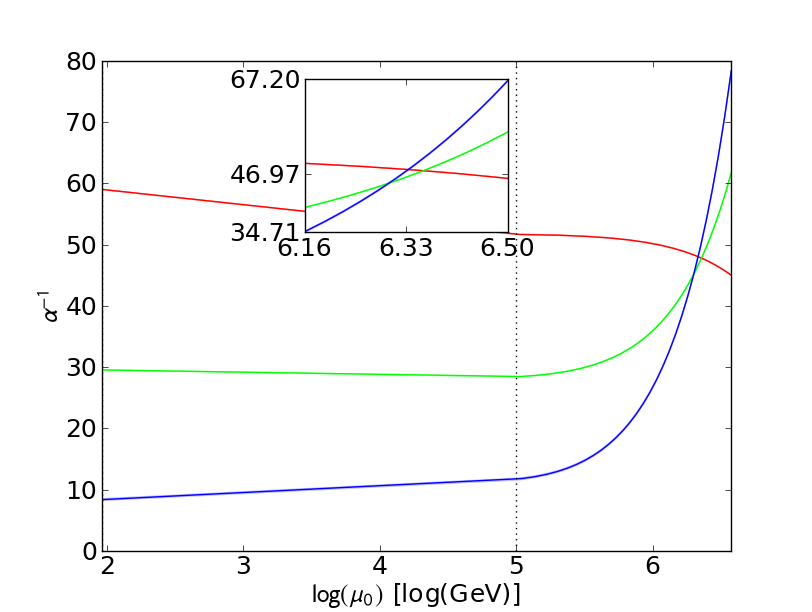
\includegraphics[width=9cm]{figs/1ed-5gev.png}
\caption[]{Plot of $\alpha_1$ (red line, top at $\mu = M_Z$), $\alpha_2$ (green) and $\alpha_3$ (blue, bottom at $\mu = M_Z$) in the ED-MSSM with 1 extra dimension, with $\mu_0 = 5$ GeV (vertical dashed line) and $M_\mathrm{SUSY} = 0$ implied. Although it looks like the couplings unify, when zooming into the unification area (inset graph) the unification is not within error. Also, $\overrightarrow{\chi}^2 (M_\mathrm{GUT}) = 659$, proving unification does not exist at this value of $\mu_0$.}
\label{fig:ed-mssm-ddg}
\end{center}
\end{figure}

Figure \ref{fig:ed-mssm-ddg} reproduces a figure in \textit{Dudas, Dienes and Gherghetta} by fixing $\mu_0 = 5$ GeV. It is hinted in the paper that the unification at this energy is approximate, but still allows the possibility of such 'low-energy' unification. By `zooming' into the area of unification we find that the couplings do not unify within error, and that the possibility of unification is highly unlikely. Furthermore, a value of $\overrightarrow{\chi}^2 (M_\mathrm{GUT}) = 659$ provides quantitative proof that unification at this energy is not possible.

\begin{figure}[th]
\begin{center}
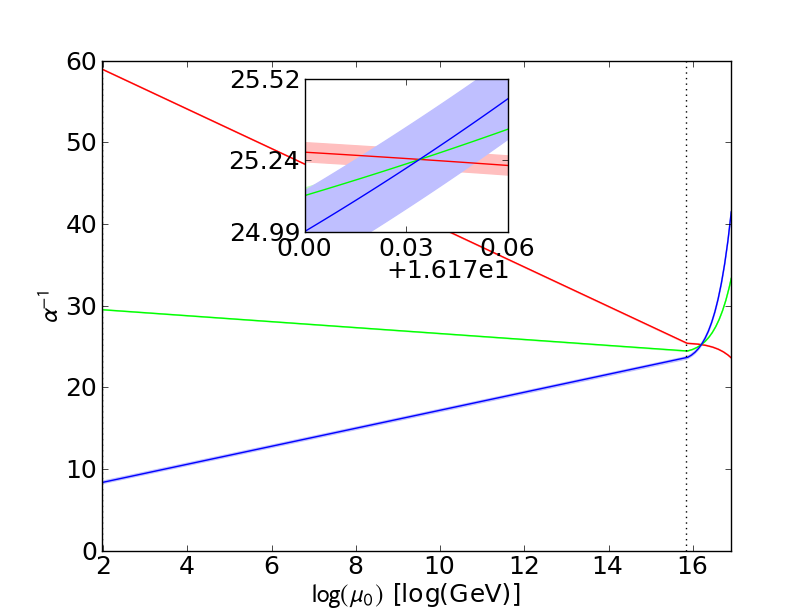
\includegraphics[width=9cm]{figs/1ed-1param-fit.png}

\begin{tabular}{c|cc|r}
$\mu_0$ [log(GeV)] & $M_\mathrm{GUT}$ [log(GeV)] & $\alpha^{-1}_\mathrm{GUT}$ & $\overrightarrow{\chi}^2 (M_\mathrm{GUT})$ \\
\hline
$15.8 \pm 0.2$ & 16.5 & 25.2 & $1.92 \times 10^{-3}$ \\
\end{tabular}

\caption[]{Plot of $\alpha_1$ (red line, top at $\mu = M_Z$), $\alpha_2$ (green) and $\alpha_3$ (blue, bottom at $\mu = M_Z$) in the ED-MSSM with 1 extra dimension, produced by allowing $\mu_0$ (dashed vertical line) to vary and minimising $\overrightarrow{\chi}^2 (M_\mathrm{GUT})$, together with a table of values used to produce the plot. All values except $\mu_0$ in the table are to 3 significant figures when $\mu_0$ takes its central value. Experimental errors are shown as lightly shaded regions around the central value.}
\label{fig:ed-mssm-fit}
\end{center}
\end{figure}

To see which values of $\mu_0$ \textit{do} admit unification, the value of $\mu_0$ was allowed to vary and $\overrightarrow{\chi}^2 (M_\mathrm{GUT})$ was minimised: the results of this analysis are found in Figure \ref{fig:ed-mssm-fit}. As can be seen from the figure, unification occurs at similar energies to those of the normal MSSM, although the unification scale is actually pushed to higher energy. 

\begin{figure}[th]
\begin{center}
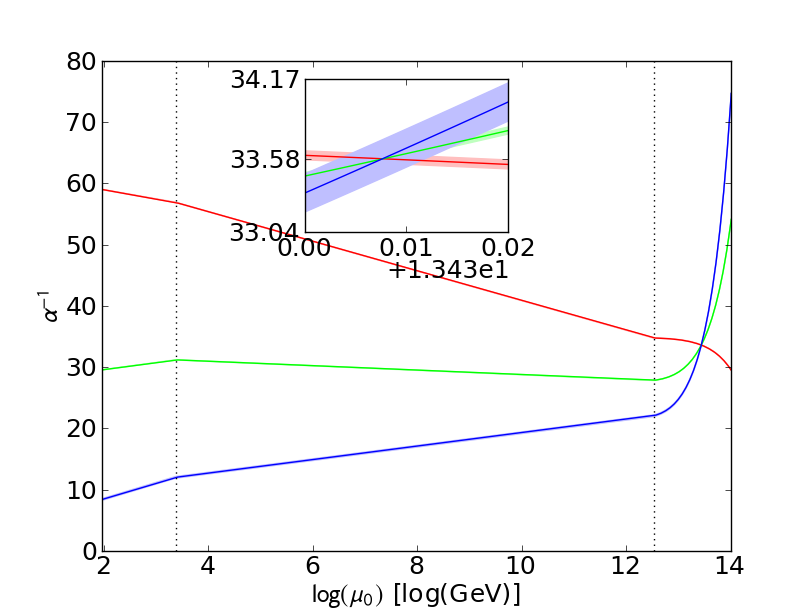
\includegraphics[width=9cm]{figs/1ed-2param-fit.png}

\begin{tabular}{cc|cc|r}
$M_\mathrm{SUSY}$ [log(GeV)] & $\mu_0$ [log(GeV)] & $M_\mathrm{GUT}$ [log(GeV)] & $\alpha^{-1}_\mathrm{GUT}$ & $\overrightarrow{\chi}^2 (M_\mathrm{GUT})$ \\
\hline
$3.38 \pm 0.04$ & $12.53\pm 0.06$ & 13.5 & 33.6 & 0.0291 \\
\end{tabular}

\caption[]{Plot of $\alpha_1$ (red line, top at $\mu = M_Z$), $\alpha_2$ (green) and $\alpha_3$ (blue, bottom at $\mu = M_Z$) in the ED-MSSM with 1 extra dimension, allowing both $M_\mathrm{SUSY}$ and $\mu_0$ (dashed vertical lines) to vary and minimising $\overrightarrow{\chi}^2 (M_\mathrm{GUT})$, together with a table of values for which $\overrightarrow{\chi}^2 (M_\mathrm{GUT})$ is minimised. All values except $M_\mathrm{SUSY}$ and $\mu_0$ in the table are to 3 significant figures when $M_\mathrm{SUSY}$ and $\mu_0$ take their central values. Experimental errors are shown as lightly shaded regions around the central value.}
\label{fig:ed-2param-fit}
\end{center}
\end{figure}

In the paper by \textit{Dudas, Dienes and Gherghetta} supersymmetry is assumed to be manifest at low energy (i.e. $M_\mathrm{SUSY} \leq M_Z$). Although this was the conclusion for the 1-loop MSSM (Figure \ref{fig:mssm-fp}a), it is reasonable to suggest that $M_\mathrm{SUSY}$ is another free parameter of this theory. We therefore allowed $M_\mathrm{SUSY}$ to vary as well as $\mu_0$ (still minimising $\overrightarrow{\chi}^2 (M_\mathrm{GUT})$); the results of this analysis are shown in Figure \ref{fig:ed-2param-fit}. From our analysis we see that the 1-loop MSSM gave an unphysical result when $M_\mathrm{SUSY}$ was the only parameter to freely vary (Figure \ref{fig:mssm-fp}a), but when extra dimensions are added to the theory the value of $M_\mathrm{SUSY}$ takes a value similar to our two-loop MSSM (Figures \ref{fig:mssm-fp}b and \ref{fig:ed-2param-fit}). 

The analysis also shows that the unification scale $M_\mathrm{GUT}$ has been lowered by 3 orders of magnitude, down to $\sim 10^{13}$ GeV. This value predicts a lower value for the proton lifetime than experimental measures allow (See Eq. \ref{eqn:proton-limit}). As postulated by Dudas, Dienes and Gherghetta, the inclusion of higher dimensions could allow a way of suppressing proton decay; for instance, if we impose Kaluza-Klein selection rules (e.g. allowing only odd Kaluza-Klein excitations for a particular particle) then we can suppress proton decay and keep the lower value for $M_\mathrm{GUT}$ \cite{gherghetta}.

\begin{figure}[th]
\begin{center}
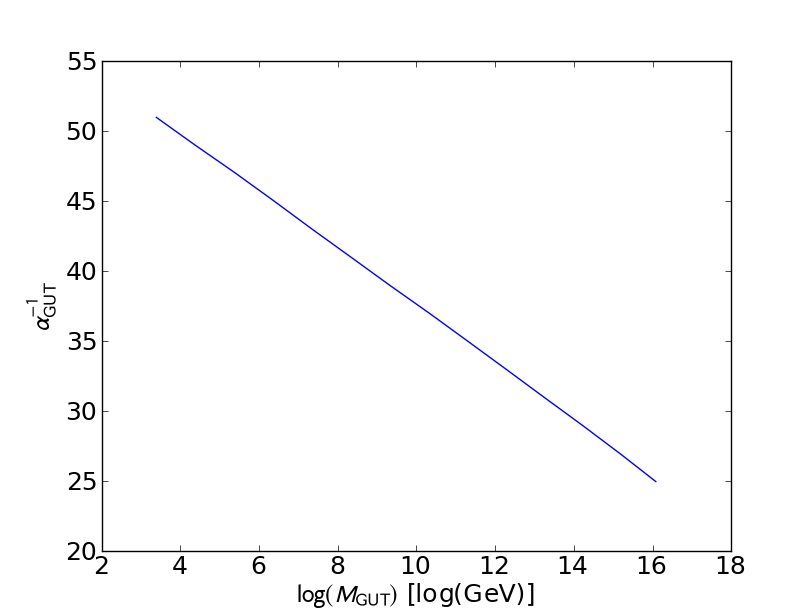
\includegraphics[width=9cm]{figs/gut-variance.png}

\caption[]{Plot of $\log(M_\mathrm{GUT})$ against $\alpha_\mathrm{GUT}^{-1}$, found by varying $\log(\mu_0)$ (which is proportional to $\alpha_\mathrm{GUT}^{-1}$). For this plot, $M_\mathrm{SUSY} = 0$. This plot is independent of the number of extra dimensions $\delta$.}
\label{fig:ed-gut-variance}
\end{center}
\end{figure}

The analysis has focussed on the addition of a single extra dimension only. The inclusion of more than one extra dimension does not alter values such as $M_\mathrm{GUT}$ and $\alpha_\mathrm{GUT}^{-1}$, as is demonstrated in Figure \ref{fig:ed-gut-variance}; for this reason, our analysis is independent of the number of extra dimensions and applies to any $\delta > 0$. For this reason, if the ED-MSSM is the correct theory to describe Nature, other analysis would be required to determine the number of extra dimensions that exist.

\section{Conclusions}
\label{sec:conc}

This report has taken a brief tour of some of the more prominent theoretical models in particle physics and determined whether each theory admits unification, and hence holds the possibility of becoming a Grand Unified Theory (GUT).

The Standard Model (SM) was found to give no unification, even when higher-order contributions were added to the beta function. This result showed that either unification is not a pursuable goal or that the SM must be extended with new physics to allow unification. Given that evidence already exists that the SM does not explain several physical phenomena (and that this report would be much shorter if we hadn't), we decided to pursue alternative theories.

The Minimal Supersymmetric Standard Model (MSSM) extends the SM by enforcing a transformation that transforms bosons into fermions and vice versa. This alteration doubles the number of particles in the model, but the beta function remains the same form - only constant factors are altered. The change in constants result in the MSSM unifying: a best-fit method arrived at (Figure \ref{fig:mssm-bp}):
\vspace{1em}
\singlespace
\[ M_\mathrm{SUSY} = 10^{(3.37 \pm 0.01)} \:\mathrm{GeV} \]
\[ \Rightarrow M_\mathrm{GUT} = 10^{(16.07 \pm 0.01)} \:\mathrm{GeV}\:, \quad \alpha_\mathrm{GUT}^{-1} = 25.60 \pm 0.02 \:, \quad (\overleftarrow{\chi}^2 < 0.01) \:. \]
\doublespace
The values determined are within the limits set by experimental bounds such as the proton decay lifetime and the maximum collider energy obtained so far, and due to overconstraint $\overleftarrow{\chi}^2$ can be made to be as low as $\sim 10^{-12}$. It is interesting to note that the value of $M_\mathrm{SUSY}$ is within the energy range due to be explored by the Large Hadron Collider (LHC), so it is reasonable to suggest from this analysis that supersymmetry signals are to be discovered at the LHC if the MSSM is correct.

The effect of compactified extra dimensions on the MSSM (together known as the ED-MSSM) were found to be not as important as first reported by \textit{Dudas, Dienes and Gherghetta}, despite the beta function gaining an extra `power law' term. By allowing the compactified dimensions' radius $R = 1/\mu_0$ to vary, we found that the ED-MSSM unifies best when (Figure \ref{fig:ed-mssm-fit})
\singlespace
\[ \mu_0 = 10^{(15.8 \pm 0.2)} \:\mathrm{GeV} \]
\[ \Rightarrow M_\mathrm{GUT} \approx 10^{16.5} \:\mathrm{GeV}\:, \quad \alpha_\mathrm{GUT}^{-1} \approx 25.2 \:, \quad (\overrightarrow{\chi}^2 = 1.92 \times 10^{-3}) \:. \]
\doublespace
The above analysis was conducted using an `always there' supersymmetry breaking scale $M_\mathrm{SUSY} = 0$; this is not physical, otherwise evidence of supersymmetry would have been found in other particle detectors. When $M_\mathrm{SUSY}$ was also allowed to vary, the values obtained were rather different (Figure \ref{fig:ed-2param-fit}):
\singlespace
\[ \mu_0 = 10^{(12.53 \pm 0.06)} \:\mathrm{GeV}\:, \quad M_\mathrm{SUSY} = 10^{(3.38 \pm 0.04)} \:\mathrm{GeV} \]
\[ \Rightarrow M_\mathrm{GUT} \approx 10^{13.0} \:\mathrm{GeV}\:, \quad \alpha_\mathrm{GUT}^{-1} \approx 33.6 \:, \quad (\overrightarrow{\chi}^2 = 0.0291) \:. \]
\doublespace
We note that $M_\mathrm{SUSY}$ agrees with the value determined in the MSSM, suggesting that even if supersymmetry was discovered at the LHC it would be difficult to determine if extra dimensions exist without alternative evidence. The unification energy scale $M_\mathrm{GUT}$ is below the experimental threshold for proton decay: another mechanism, such as Kaluza-Klein selection rules, is required to allow the unification scale to be this low. We also note that our analysis is independent of the number of extra dimensions added to the MSSM (Figure \ref{fig:ed-gut-variance}).

Although we have provided a thorough analysis of the ED-MSSM, the analysis was done at one-loop; it would be interesting to see whether the analysis alters significantly if two-loop contributions are added (which, in the case of the MSSM, raised $M_\mathrm{SUSY}$ to scales just beyond our current experimental bounds: see Figure \ref{fig:mssm-fp}). This is a very complicated analysis, as each of the couplings will couple to the other two as shown e.g. in the two-loops terms of Eq. \ref{eqn:mssm-beta}.

As well as this, using the BP method on the ED-MSSM could yield more accurate values on $\mu_0$ and $M_\mathrm{SUSY}$; however, it is worth noting that we have 4 degrees of freedom and three equations, leading to the possibility that the problem is overconstrained.

\vspace{1em}

A number of theories beyond the Standard Model allow for unification; at what energy that unification occurs is dependent on the theory, but it is safe to assume that the energy scale will not be experimentally obtainable in the current or next generation of particle colliders. As such, it is tentative to assume that we will not find new physics in the `desert' between our currently attainable energy scale and the unification scales hypothesised by these theories. If there really is no new physics at these energy scales, the next step is to incorporate gravity into a Grand Unified Theory to give a Theory of Everything. Based on the investigations presented here, an extra-dimensional extension to the Minimal Supersymmetric Standard Model could potentially be the first step to a Theory of Everything: however, experimental results at the Large Hadron Collider should determine whether supersymmetry is correct or whether a new description of Nature is required.

\section*{Acknowledgements}
\addcontentsline{toc}{section}{Acknowledgements}
The author would like to thank his supervisor Dr. Chris Maxwell for his invaluable time and guidance.

% Stop double spacing
%\clearpage % Clears figures and starts new page for references
\singlespace
\addcontentsline{toc}{section}{References}
\begin{thebibliography}{99}

% Introduction
\bibitem{sm-1}{P. S. Wells, \textit{Experimental Tests of the Standard Model}, Eur. Phys. J. C \textbf{33}, S1 (2004), pp. 5-20}
\bibitem{sm-2}{A. Olchevski, M. Winter, \textit{High Precision Tests of the Standard Model and Determination of the Top Quark and Higgs Boson Masses}, C. R. Physique \textbf{3} (2002), pp. 1183-1191}
\bibitem{neutrinos}{M. D. Messier, \textit{Review of Neutrino Oscillation Experiments}, Proceedings of the Flavor Physics and CP Violation Conference, Vancouver (2006)}
\bibitem{mass}{E. Saether, \textit{The Mystery of the Matter Asymmetry}, Beam Line \textbf{26}, SLAC (1996)}
\bibitem{hier}{M. C. Brak, \textit{The Hierarchy Problem in the Standard Model and Little Higgs Theories}, Masters Thesis, NIKHEF (2004)}
\bibitem{unnatural}{J. Hewett, \textit{Non-SUSY Physics Beyond the Standard Model}, Presentation at Pre-SUSY '10, Physikalische Institut, Bonn (2010); available online at \url{http://susy10.uni-bonn.de/presusy.php}}
\bibitem{amaldi}{U. Amaldi, W. de Boer, P. H. Frampton, H. F\"{u}rstenau and J. T. Liu, \textit{Consistency Checks of Grand Unified Theories}, Phys. Lett. B \textbf{281} (1992), pp. 374-382}
\bibitem{running-2}{G.M. Prosperia, M. Racitia and C. Simolo, \textit{On the Running Coupling Constant in QCD}, Progress in Particle and Nucl. Phys. \textbf{58}, 2 (2007), pp. 387-438}
\bibitem{lhp}{K. S. Babu, I. Gogoladze, M. U. Rehman and Q. Shafi, \textit{Higgs Boson Mass, Sparticle Spectrum, and the Little Hierarchy Problem in an Extended MSSM}, Phys. Rev. D \textbf{78}, 055017 (2008)}
\bibitem{mssm}{S. P. Martin, \textit{A Supersymmetry Primer}, arxiv:hep-ph/9709356v5 (2008)}
\bibitem{mssm-lhc}{P. Konar, K. T. Matchev, M. Park and G. K. Sarangi, \textit{How to Look for Supersymmetry Under the LHC Lamppost}, Phys. Rev. Lett. \textbf{105}, 221801 (2010)}
\bibitem{ed-1}{N. Arkani-Hamed, S. Dimopolous and G. Dvali, \textit{The Hierarchy Problem and New Dimensions at a Millimeter}, Phys. Lett. B \textbf{429}, 3-4 (1998), pp. 263-272}
\bibitem{ed-2}{L. Randall and R. Sundrum, \textit{Large Mass Hierarchy from a Small Extra Dimension}, Phys. Rev. Lett. \textbf{83}, 3370-3373 (1999)}
\bibitem{string}{J. G. Polchinski, \textit{String Theory}, CUP (2003), Section 10.6: Superstring Theories in 10 Dimensions}
\bibitem{gherghetta}{K. R. Dienes, E. Dudas and T. Gherghetta, \textit{Extra Spacetime Dimensions and Unification}, Phys. Lett. B \textbf{436}, 55 (1998)}
\bibitem{pdg}{K. Nakamura et al. (Particle Data Group), \textit{2010 Review of Particle Physics}, J. Phys. G \textbf{37}, 075021 (2010), Section 15: Grand Unified Theories}

% Analytical Theory
\bibitem{peskin}{M. E. Peskin and D. V. Schroeder, \textit{An Introduction to Quantum Field Theory}, Perseus Books (1995), pp. 248-249}
\bibitem{ms}{W. A. Bardeen, A. Buras, D. Duke and T. Muta, \textit{Deep-Inelastic Scattering Beyond the Leading Order in Asymptotically Free Gauge Theories}, Phys. Rev. D \textbf{18} (1978), pp. 3998-4017}
\bibitem{dr}{I. Antoniadis, C. Kounnas, K. Tamvakis, \textit{Simple Treatment of Threshold Effects}, Phys. Lett. B \textbf{119} (1982), pp. 377-380}
\bibitem{renorm-2}{A. E. Blechman, \textit{Renormalization: Our Greatly Misunderstood Friend}, Presentation at Johns Hopkins University, Baltimore (2002); available online at \url{http://www.pha.jhu.edu/~blechman/papers/renormalization/renormalization.html}}
\bibitem{bogoliubov}{N. N. Bogoliubov and D. V. Shirkov, \textit{Introduction to the Theory of Quantized Fields}, Wiley (1959), Chapter VIII: The Renormalisation Group}

% Computational Theory
\bibitem{scipy}{\texttt{numpy} and \texttt{scipy} are available from \url{http://www.scipy.org/}}
\bibitem{pylab}{J. Hunter, D. Dale, M. Droettboom, \textit{matplotlib - python plotting}, \url{http://matplotlib.sourceforge.net/}}

% Standard Model
\bibitem{sm}{F. E. Close, I. G. Halliday, T. Jones and C. Maxwell, Proceedings of the School for Young High Energy Physicists, Rutherford Appleton Laboratory, Oxford (1993)}
\bibitem{sm-renorm}{H. Arason, D. J. Castano, B. Keszthelyi, S. Mikaelian, E. J. Piard, P. Ramond, and B. D. Wright, \textit{Renormalization-Group Study of the Standard Model and its Extensions: I. The Standard Model}, Phys. Rev. D \textbf{46} (1992), pp. 3945}
\bibitem{5thirds}{H. Georgi, H. R. Quinn, S. Weinberg, \textit{Hierarchy of Interactions in Unified Gauge Theories}, Phys. Rev. Lett. \textbf{33} (1984), pp. 451-454}
\bibitem{b}{M. B. Einhorn and D. R. T. Jones, \textit{The Weak Mixing Angle and Unification Mass in Supersymmetric SU(5)}, Nucl. Phys. B \textbf{196} (1982), pp. 475-488}

% MSSM
\bibitem{mssm-renorm}{D. J. Castano, E. J. Piard and P. Ramond, \textit{Renormalization-Group Study of the Standard Model and its Extensions: II. The Minimal Supersymmetric Standard Model}, Phys. Rev. D \textbf{49} (1994), pp. 4882-4901} 
\bibitem{yukawa}{G. Amelino-Cameliab, D. Ghilencea and G. G. Ross, \textit{The Effect of Yukawa Couplings on Unification Predictions and the Non-Perturbative Limit}, Nuc. Phys. B \textbf{528}, 1-2 (1998), pp. 35-58}
\bibitem{lhc-1}{ATLAS Collaboration, \textit{ATLAS Detector and Physics Performance, Technical Design Report, Vol. II}, CERN-LHCC-99-15 (1999)}
\bibitem{lhc-2}{CMS Collaboration, \textit{CMS, the Compact Muon Solenoid: Technical Proposal}, CERN-LHCC-94-38 (1994)}

% ExD
\bibitem{kk}{P. S. Wesson, \textit{Space-Time-Matter: Modern Kaluza-Klein Theory}, World Scientific (1998), Chapter 1.5: Kaluza-Klein Theory}
\bibitem{black-holes-lhc}{The CMS Collaboration, \textit{Search for Microscopic Black Hole Signatures at the Large Hadron Collider}, Phys. Lett. B, \textbf{697}, 5 (2011), pp. 434-453}
\bibitem{kk-exp}{A. M\"{u}ck, \textit{The Standard Model in 5D: Theoretical Consistency and Experimental Constraints}, Doctoral Thesis, Bayerischen Julius-Maximilians-Universit\"{a}t W\"{u}rzburg (2004)}

\end{thebibliography}

% Start appendices
\newpage
\appendix

\part*{Appendices}
\addcontentsline{toc}{part}{Appendices}

\section{Comparison of Integration Methods}
\label{apx:tic}

In this study two methods were used to integrate differential equations. The first method was based on Taylor series (and is herein referred to as the Taylor method): The Taylor series to $\alpha^{-1}_i (\mu)$ is approximated, and then we step along the function using the definition of ${d \alpha^{-1}_i}/{d \mu}$ from Eq. \ref{eqn:rg-i}. Explicitly, the formula used is
\[
\alpha_i^{-1} (\mu + \Delta \mu) = \alpha_i^{-1} (\mu) + \left(\dfrac{d \alpha_i^{-1}}{d \mu}\right) \Delta \mu \:.
\]

The second method used the \texttt{odeint} routine of the Python \texttt{scipy} module; this routine uses a mixture of Adams and BDF methods to determine the solutions (see, for example: Astic, Bahain and Jerosolimski, \textit{The mixed Adams-BDF Variable Step Size Algorithm to Simulate Transient and Long-Term Phenomena in Power Systems}, IEEE Transactions on Power Systems \textbf{9}, 2 (1994)).

\begin{figure}[th]
\begin{center}

\begin{tabular}{cc}
(a) 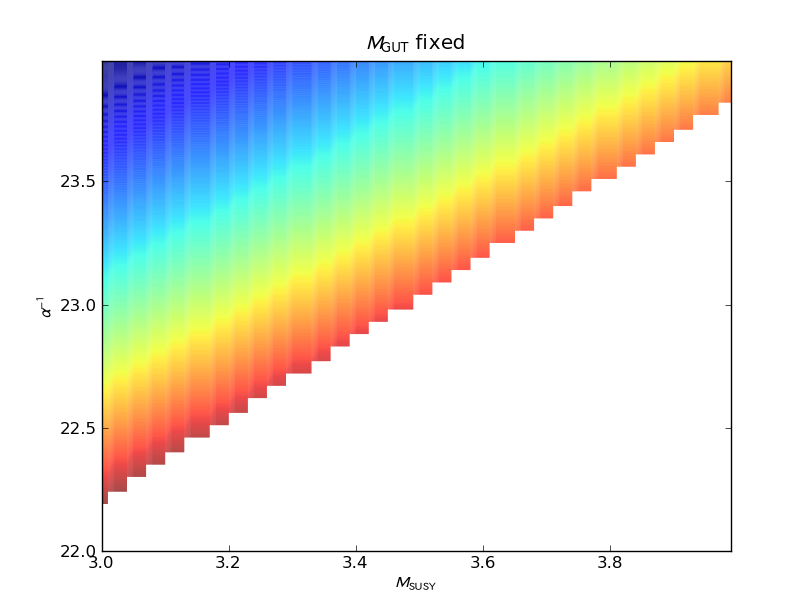
\includegraphics[width=6.85cm]{figs/int-taylor.png} &
(b) 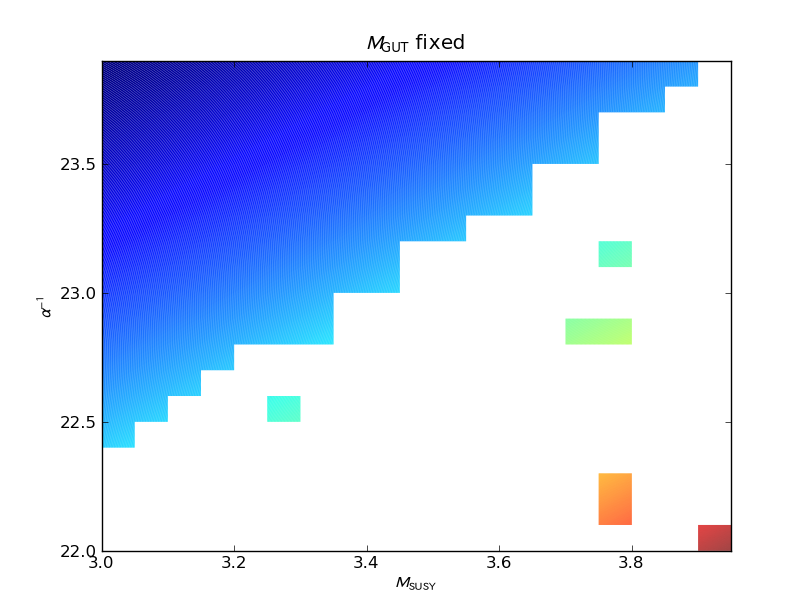
\includegraphics[width=6.85cm]{figs/int-odeint.png}
\end{tabular}

\caption[]{Comparison of integration method stability as parameters become unsolvable. (a) Taylor method. (b) \texttt{odeint} routine. White areas denote where each method could not solve for the given parameters. As can be seen from the plots the Taylor method provides no false values if it is given unsolvable parameters, whereas the \texttt{odeint} routine sometimes incorrectly `solves' unsolvable parameters.}
\label{fig:int-comparison}
\end{center}
\end{figure}

Both methods produced similar numerical results in the vast majority of cases. The Taylor method was more stable (see Figure \ref{fig:int-comparison}), but took longer to calculate than the \texttt{odeint} routine. Because of their features, both methods were used in the study: when speed was required and the parameters used were well away from the unsolvable boundary, the \texttt{odeint} method was used; otherwise, the Taylor method was used.

\section{Error Propagation}
\label{apx:errors}

The couplings in the Standard Model (SM) are given by (Eq. \ref{eqn:coupling-def})
\[
\alpha_1^{-1} = \dfrac{3}{5} \dfrac{\cos^2 \theta_W}{a} \:, \quad
\alpha_2^{-1} = \dfrac{\sin^2 \theta_W}{a} \:, \quad
\alpha_3^{-1} = \dfrac{1}{a_s}
\]
and using the world-averaged values (Eq. \ref{eqn:world-vals})
\begin{align}
a^{-1} (M_Z) &= 127.91 \pm 0.02 \nonumber \\
\sin^2 \theta_W (M_Z) &= 0.2312 \pm 0.0002 \nonumber \\
a_s (M_Z) &= 0.119 \pm 0.002 \nonumber
\end{align}
we can determine the running of the couplings. Using $\sigma[x]$ to denote the error in $x$, the errors in a function $f(x_1, x_2, ..., x_n)$ has error
\[
\sigma[f(x_1, x_2, ..., x_n)] = \sqrt{\sum_{i=1}^{n} \left( \frac{\partial f}{\partial x_i} \right)^2 \sigma[x_i]^2}
\]
In this case, the errors in each $\alpha_i^{-1}$ are given by
\begin{align}
\sigma[\alpha_1^{-1}] &= \sqrt{\left(\dfrac{3 a^{-1}}{5} \dfrac{\sigma[\sin^2 \theta_W]}{\sqrt{\sin^2 \theta_W}} \right)^2 + \left( \dfrac{\alpha_1^{-1} \sigma[a^{-1}]}{a^{-1}} \right)^2 } \nonumber \\
\sigma[\alpha_2^{-1}] &= \alpha_2^{-1} \sqrt{ \left( \dfrac{\sigma[\sin^2 \theta_W]}{\sin^2 \theta_W} \right)^2 + \left( \dfrac{\sigma[a^{-1}]}{a^{-1}} \right)^2 } \nonumber \\
\sigma[\alpha_3^{-1}] &= \dfrac{\alpha_3^{-1}}{a_s} \sigma[a_s] \nonumber
\end{align}
where $\sigma[\sin^2 \theta_W]$, $\sigma[a^{-1}]$ and $\sigma[a_s]$ are defined in Eq. \ref{eqn:world-vals}. This implies that (Eq. \ref{eqn:couplingvals})
\[
\alpha_1^{-1} (M_Z) = 59.00 \pm 0.03 \:, \quad
\alpha_2^{-1} (M_Z) =  29.52 \pm 0.03 \:, \quad
\alpha_3^{-1} (M_Z) =  8.3 \pm 0.1
\]
\clearpage
\section{The MCLM Algorithm}
\label{apx:mclm}

To determine the global minimum of a function of many variables, a hybrid convergence algorithm was used: the Monte-Carlo Levenberg-Marquardt (MCLM) algorithm. This algorithm uses a mixture of stochastic and convergence methods to quickly obtain a global minimum.

The algorithm runs a number of trials: at the start of each trial, each of the parameters of the function are randomly set between a given range of possible values. These initial conditions are then passed to a Levenberg-Marquardt algorithm (see, for example: Jorge and Wright, \textit{Numerical Optimisation}, Springer, 2nd Ed. (2006)), which converges to a local minimum for that set of initial conditions. If the local minimum is lower than any other minimum calculated so far, it is considered the global minimum.

As the number of trials increases, the likelihood that the current minimum is the global minimum increases. Although this will never reach certainty, by running enough trials the confidence level can be increased.

\end{document}